\documentclass[a4paper]{article}
\usepackage[english]{babel}
\usepackage[utf8]{inputenc}
\usepackage{textcomp}
\usepackage{amsmath}
\usepackage{gensymb}
\usepackage{physics}
\usepackage{graphicx}
\usepackage[colorinlistoftodos]{todonotes}
\usepackage{xcolor}
\usepackage{array}
\usepackage{tabularx}
\usepackage{tikz}
\usepackage{framed}
\usepackage{xfrac}
\usepackage[most]{tcolorbox}
\usepackage{fix-cm}
\usepackage[margin=0.5in]{geometry}
\usetikzlibrary{quotes,angles}
\usetikzlibrary{decorations.pathreplacing}
\usetikzlibrary{calc}

\let\phi\varphi
\let\bf\textbf
\colorlet{shadecolor}{orange!15}
\def\centerarc[#1](#2)(#3:#4:#5){\draw[#1] ($(#2)+({#5*cos(#3)},{#5*sin(#3)})$) arc (#3:#4:#5)}

\title{Linear Momentum \& Collisions}
\author{OpenStax University Physics Vol. 1}

\begin{document}
\setcounter{section}{9}
\maketitle
\subsection{Linear Momentum}
The momentum $p$ of an object is the product of its mass and its velocity
\begin{equation}
    \displaystyle \vec{p} = m\vec{v}
\end{equation}
Unlike kinetic energy, momentum depends equally on an object's mass and velocity. For example, the average speed of an air molecule at room temperature is $\approx 500$ ms$^{-1}$, with an average molecular mass of $6 \cdot 10^{-25}$ kg; its momentum is thus:
\begin{center}
    $\displaystyle p_{mol} = (6\cdot 10^{-25}\text{ kg})(500\text{ ms}^{-1}) = 3 \cdot 10^{-22} \text{ kg\:ms}^{-1}$
\end{center}

\subsection{Impulse \& Collisions}
Suppose you apply a force on a free object for some amount of time, clearly the larger the force, the larger the change in momentum of the object will be. Alternatively, the more time you spend applying the force, the large the change in momentum will be. The amount by which the object's motion changes is therefor proportional to the magnitude of the force, and also to the time interval over which the force is applied.
\vspace{2mm}\\
\bf{Impulse ($\vec{J}$)} - The product of a force and a time interval over which that force acts
\vspace{1mm}\\
Let $\vec{F}(t)$ be the force applied to an object over some differential time interval $dt$. The resulting impulse on the object is defined as:
\begin{equation}
    d\vec{J} = \vec{F}(t)dt
\end{equation}
The total impulse over the time interval $t_f - t_i$ is:
\begin{equation}
    \vec{J} = \int_{t_i}^{t_f}d\vec{J} \ \boldsymbol{\to} \ \vec{J} = \int_{t_i}^{t_f}\vec{F}(t)dt
\end{equation}
Together, these equations say that when a force is applied for an infinitesimal time interval $dt$, it causes and infinitesimal impulse $d\vec{J}$, and that the total impluse given to the object is defined to be the sum of all these infinitesimal impulses.

To calculate the impulse, we need to know the force function $F(t)$ which we often don't. However recall that the average value of a function over some interval is calculated by the equation below where $\Delta x = x_f - x_i$
\begin{center}
    $\displaystyle f(x)_{ave} = \frac{1}{\Delta x}\int_{x_i}^{x_f}f(x)dx$
\end{center}
Applying this to the time-dependent force function, we obtain:
\begin{equation}
    \vec{F}_{ave} = \frac{1}{\Delta t}\int_{t_i}^{t_f}\vec{F}(t)dt
\end{equation}
Therefore, based on equation 3:
\begin{equation}
    \vec{J} = \vec{F}_{ave}\Delta t
\end{equation}
The impulse of an object can be calculated even if the details of the force as a function of time are not known; only average force is needed.
\vspace{1mm}\\
To calculate impulse, a useful result can be obtained by writing force in equation 3 as $\vec{F}(t) = m\vec{a}(t)$:
\begin{center}
    $\displaystyle \vec{J} = \int_{t_i}^{t_f}\vec{F}(t)dt = m\int_{t_i}^{t_f}\vec{a}(t)dt = m[\vec{v}(t_f) - \vec{v}_i]$
\end{center}
For constant force $\vec{F}_{ave} = \vec{F} = m\vec{a}$, this simplifies to 
\begin{center}
    $\vec{J} = m\vec{a}\Delta t = m\vec{v}_f - m\vec{v}_i = m(\vec{v}_f - \vec{v}_i)$
\end{center}
This can be rewritten as
\begin{equation}
    \vec{J} = m\Delta\vec{v}
\end{equation}
\newpage

\noindent\bf{Effect of Impulse}
\vspace{2mm}\\
Since impulse is a force acting for some amount of time, it causes an object's motion to change. Because $m\vec{v}$ is the momentum of a system, $m\Delta\vec{v}$ is the change of momentum $\Delta\vec{p}$. This relation is called the impulse-momentum theorem.
\vspace{1mm}\\
\bf{Impulse-Momentum Theorem} - An impulse applied to a system changes the system's momentum, and that change in momentum is exactly equal to the impulse that was applied:
\begin{equation}
    \vec{J} = \Delta\vec{p}
\end{equation}
There are two crucial concepts in the impulse-momentum theorem:
\begin{enumerate}
    \item Impulse is a vector quantity; an impulse of $(-10$N$\cdot$s$)\hat{i}$ is very different from an impulse of $(+10$N$\cdot$s$)\hat{i}$; they cause completely opposite changes of momentum
    \item An impulse does not cause momentum, it causes a change in the momentum of an object. Thus, you must subtract the initial momentum from the final momentum, taking careful account of the signs of the momentum vectors
\end{enumerate}
\begin{shaded}
    \underline{\bf{Example 9.3} Moving the Enterprise}
    \vspace{2mm}\\
    When Captain Picard commands "Take us out", the starship Enterprise starts from rest to a final speed of $v_f = 7.5 \cdot 10^7$ms$^{-1}$. Assuming this maneuver is completed in 60 s, what average force did the impulse engines apply to the ship? The mass of the Enterprise can be estimated as $2 \cdot 10^9$ kg.
    \vspace{1mm}\\
    Because the problem only involves one direction, only the scalar form of the impulse-momentum theorem is needed, which is:\\
    $\Delta p = J\ $ with $\ \Delta p = m \Delta v\ $ and $\ J = F \Delta t$\\
    Equating these expressions gives: $F \Delta t = m \Delta v$\\
    Solving for the magnitude of the force and inserting the given values leads to:\\
    $\displaystyle F = \frac{m \Delta v}{\Delta t} = \frac{(2 \cdot 10^9\text{ kg})(7.5 \cdot 10^7 \text{ ms}^{-1})}{60\text{ s}} = 2.5 \cdot 10^{15}$ N
\end{shaded}
\bf{Momentum \& Force}
\vspace{1mm}\\
In equation 3, an important relationship was obtained
\begin{equation}
    \vec{F}_{ave} = \frac{\Delta\vec{p}}{\Delta t}
\end{equation}
The average force applied to an object is equal to the change in momentum that the force causes, divided by the time interval over which this change in momentum occurs. This relationship is very useful in situations where the collision time $\Delta t$ is small but measurable.

For a continuously changing momentum - due to a continuously changing force - this becomes a powerful conceptual tool. In the limit $\Delta t \to dt$, equation 2 becomes
\begin{equation}
    \vec{F} = \frac{d\vec{p}}{dt}
\end{equation}
This says that the rate of change of the system's momentum is exactly equal to the net applied force, this is Newton's second law written in terms of momentum rather than acceleration
\begin{center}
    $\displaystyle \vec{F} = \frac{d\vec{p}}{dt} = \frac{d(m\vec{v})}{dt} = m\frac{d\vec{v}}{dt} = m\vec{a}$
\end{center}
The assumption of constant mass allowed us to pull $m$ out of the derivative. If the mass is not constant, we cannot use this form of the second law, and must instead start from equation 3. Thus, one advantage to expressing force in terms of changing momentum is that it allows for the mass of the system to change, as well as the velocity
\vspace{1mm}\\
\noindent The net external force on a system is equal to the rate of change of the momentum of that system caused by a force:
\begin{center}
    $\displaystyle \vec{F} = \frac{d\vec{p}}{dt}$
\end{center}

\begin{shaded}
    \underline{\bf{Example 9.5} Calculating Force: Venus Williams' Tennis Serve}
    \vspace{2mm}\\
    During the 2007 French Open, Venus Williams hit the fastest recorded serve in a premier women's match, reaching a speed of 58 ms$^{-1}$. What is the average force exerted on the 0.057 kg tennis ball by Venus Williams' racquet? Assume that the ball's speed just after impact is 58 ms$^{-1}$, that the horizontal component of the velocity before impact is negligible, and that the ball remained in contact with the racquet for 5.0 ms.
    \vspace{1mm}\\
    To determine the change in momentum, insert the values for the initial and final velocities into the equation:\\
    $\Delta p = m\Delta v = m(v_f - v_i) \ \to \ \Delta p = (0.057$ kg$)(58$ ms$^{-1} - 0$ ms$^{-1}) = 3.3$ kg\;ms$^{-1}$\\
    Now the magnitude of the net external force can be determined by using:\\
    $\displaystyle F = \frac{\Delta p}{\Delta t} = \frac{3.3\text{ kg\;ms}^{-1}}{5.0 \cdot 10^{-3}\text{s}} = 6.6 \cdot 10^2$ N
\end{shaded}

\newpage
\subsection{Conservation of Linear Momentum}
Recall Newton's third law: when two objects of masses $m_1$ and $m_2$ interact, the force that object 2 applies to object 1 is equal in magnitude and opposite in direction to the force that object 1 applies on object 2
\vspace{1mm}\\
Let $\vec{F}_{2 \to 1} =$ The force on $m_1$ from $m_2$, and $\vec{F}_{1 \to 2} =$ The force on $m_2$ from $m_1$
\begin{equation}
    \begin{aligned}
        \vec{F}_{2 \to 1} = -\vec{F}_{1 \to 2}\\
        m_1\vec{a}_1 = -m_2\vec{a}_2
    \end{aligned}
\end{equation}
The two forces do not cancel because they are applied to different objects. $F_{2 \to 1}$ causes $m_1$ to accelerate, and $F_{1 \to 2}$ causes $m_2$ to accelerate. 

Although the magnitudes of the forces on the objects are the same, the accelerations are not because the masses are different:
\begin{center}
    $\displaystyle \frac{d\vec{v}_1}{dt} \neq \frac{d\vec{v}_2}{dt}$
\end{center}
However, the products of the mass and the change of velocity are equal in magnitude
\begin{equation}
    m_1\frac{d\vec{v}_1}{dt} = -m_2\frac{d\vec{v}_2}{dt}
\end{equation}
Because of the interaction, each object ends up getting its velocity changed by an amount $dv$. The interaction occurs over a time interval $dt$, which means that the change in velocities also occurs over $dt$. This time interval is the same for each object.

Assuming that the masses of the objects do not change during the interaction, we can pull the masses inside the derivative
\begin{equation}
    \frac{d}{dt}(m_1\vec{v}_1) = - \frac{d}{dt}(m_2\vec{v}_2)
\end{equation}
Thus,
\begin{equation}
    \frac{d\vec{p}_1}{dt} = -\frac{d\vec{p}_2}{dt}
\end{equation}
The rate at which momentum changes is the same for both objects. Their masses are different, and the changes in velocity are different, but the rate of change of the product of $m$ and $\vec{v}$ are the same. This means that during the interaction of the two objects $m_1$ and $m_2$, both objects have their momentum changed; but those changes are identical in magnitude, and opposite in sign.
\vspace{1mm}\\
Rewriting equation 13 in a more suggestive form:
\begin{equation}
    \frac{d\vec{p}_1}{dt} + \frac{d\vec{p}_2}{dt} = 0
\end{equation}
During the interaction, although object 1's momentum changes, and object 2's momentum also changes, these two changes cancel each other out, so that the total change of momentum of the two objects together is zero.
\vspace{1mm}\\
Since the total combined momentum of the two objects together never changes, we could write:
\begin{equation}
    \frac{d}{dt}(\vec{p}_1 + \vec{p}_2) = 0
\end{equation}
From which it follows that:
\begin{equation}
    \vec{p}_1 + \vec{p}_2 = \text{constant}
\end{equation}
The total momentum of the system before and after the collision remains the same
\vspace{1mm}\\
Generalizing this result to $N$ objects:
\begin{equation}
    \begin{aligned}
        \vec{p}_1 + \vec{p}_2 + \vec{p}_3 + ... + \vec{p}_N = \text{constant}\\
        \sum_{j=1}^{N}\vec{p}_j = \text{constant}
    \end{aligned}
\end{equation}
This equation is the definition of the total or net momentum of a system of $N$ interacting objects, along with the statement that the total momentum of a system of objects is conserved.

\newpage
\noindent\bf{Requirements for Momentum Conservation} - A system must meet two requirements for its momentum to be conserved
\begin{enumerate}
    \item The mass of the system must remain constant during the interaction.\\
    As the objects interact, they may transfer mass from one to another, but any mass one object gains is balanced by the loss of that mass from another. The total mass of the system remains unchanged with respect to time:
    \begin{align*}
        \displaystyle \bigg[\frac{dm}{dt}\bigg]_{\text{sys}} = 0
    \end{align*}
    \item The net external force on the system must be zero\\
    As the objects collide, or explode, and move around, they exert forces on each other. All of these forces are internal to the system and are balanced by another equal and opposite internal force. Internal forces cannot change the total momentum of a system because the changes sum to zero. If there is some external force that acts on all of the objects, then this force changes the momentum of the system as a whole. For the momentum of a system to be conserved, we must have:
    \begin{align*}
        \displaystyle \vec{F}_{ext} = \vec{0}
    \end{align*}
\end{enumerate}
A system of objects that meets these requirements is said to be a closed system (also called an isolated system)
\vspace{2mm}\\
\bf{Law of Conservation of Momentum} - The total momentum of a closed system is conserved:
\begin{center}
    $\displaystyle \sum_{j=1}^{N}\vec{p}_j =$ constant
\end{center}
\vspace{2mm}

\begin{shaded}
    \underline{\bf{Example 9.6} Colliding Carts}
    \vspace{2mm}\\
    Two carts in a physics lab roll on a level track with negligible friction. These carts have small magnets at their ends, so that when they collide, they stick together. The first cart has a mass of $m_1 = 675$ g and is rolling at $v_1 = 0.75$ ms$^{-1}$ to the right; the second has a mass of $m_2 = 500$ g and is rolling at $v_2 = 1.33$ ms$^{-2}$, also to the right. After the collision, what is the velocity of the two joined carts?
    \vspace{1mm}\\
    The conservation of momentum is: $\vec{p}_f = \vec{p}_i$\\
    Define the direction of their intitial velocity vectors to be in the $+x$ direction.\\
    The initial momentum is then: $\vec{p}_i = m_1v_1\hat{i} + m_2v_2\hat{i}$\\
    The final momentum of the now-linked cart is: $\vec{p}_f = (m_1 + m_2)\vec{v}_f$\\
    Equating gives: $\displaystyle (m_1 + m_2)\vec{v}_f = m_1v_1\hat{i} + m_2v_2\hat{i} \ \boldsymbol{\to} \ \vec{v}_f = \Big(\frac{m_1v_1 + m_2v_2}{m_1 + m_2}\Big)\hat{i}$\\
    Substituting the given values: $\displaystyle \vec{v}_f = \bigg[\frac{(0.675\text{ kg})(0.75\text{ ms}^{-1}) + (0.5\text{ kg})(1.33\text{ ms}^{-1})}{1.175\text{ kg}}\bigg]\hat{i} = (0.997\text{ ms}^{-1})\hat{i}$
\end{shaded}

%%% ADD MORE EXAMPLES FROM OPENSTAX 9.3 %%%

\newpage
\subsection{Types of Collisions}
Although momentum is conserved in all interactions, not all interactions (collisions or explosions) are the same. Possibilities include:
\begin{itemize}
    \item A single object can explode into multiple objects (explosions)
    \item Multiple objects can collide and bounce off each other, called an \underline{elastic collision}, resulting in the same kinetic energy of the system before and after the collision
    \item Multiple objects can collide and the system looses kinetic energy called an \underline{inelastic collision}. One such case is where the two objects stick together, forming a single object. 
\end{itemize}
\bf{Explosions}
\vspace{1mm}\\
A single object may break apart into two or more pieces. These can be difficult to analyze if the number of fragments after the collision is more than about 3 or 4 however, the total momentum of the system before and after the explosion is identical.

If the object is initially motionless, then the system has no momentum and no kinetic energy. After the explosion, the net momentum of all the pieces of the object must sum to zero due to conservation of momentum. However, the system will have a great deal of kinetic energy after the explosion although it had none before. Although the momentum of the system is conserved in an explosion, the kinetic energy is not. This interaction - one object becoming many with an increase in the kinetic energy of the system - is called an explosion.
\vspace{2mm}\\
\bf{Inelastic}
\vspace{1mm}\\
When two objects collide with each other and stick together, forming a single composite object. The total mass of this composite object is the sum of the masses of the original objects, and the new single object moves with a velocity dictated by the conservation of momentum. Although the total momentum of the system remains constant, the kinetic energy decreases, this type of collision is called an inelastic collision.

Any collision where the objects stick together will result in the maximum loss of kinetic energy ($k_f$ will be a minimum). Such a collision is called \underline{perfectly inelastic}. 
\begin{itemize}
    \item If $0 < K_f < K_i$, the collision is inelastic
    \item If $K_f$ is the lowest energy, or the energy lost by both objects is the most, the collision is perfectly inelastic (objects stick together)
    \item If $K_f = K_i$, the collision is elastic
\end{itemize}
\bf{Elastic}
\vspace{1mm}\\
When two or more objects approach each other, collide, and bounce off each other, moving away from each other at the same relative speed at which they approached each other. In this case, the total kinetic energy of the system is conserved, such an interaction is called elastic

\begin{shaded}
    \underline{\bf{Example 9.10} Formation of a Deuteron}
    \vspace{2mm}\\
    A proton (mass $1.67 \cdot 10^{-27}$ kg) collides with a neutron - with essentially the same mas as the proton - to form a particle called a deuteron. What is the velocity of the deuteron if it is formed from a proton moving with a velocity of $7.0 \cdot 10^6$ ms$^{-1}$ to the left and a neutron moving with velocity $4.0 \cdot 10^6$ ms$^{-1}$ to the right?
    \vspace{1mm}\\
    Treat the particles as having identical masses $M$. Use the subscripts $p, n,$ and $d$ for proton, neutron, and deuteron. This is a one-dimensional problem so we have\\
    $Mv_p - Mv_n = 2Mv_d$\\
    The masses divide out:
    \begin{align*}
        v_p - v_n = 2v_d\\
        7.0 \cdot 10^6 \text{ ms}^{-1} - 4.0 \cdot 10^6 \text{ms}^{-1} = 2v_d\\
        v_d = \frac{3 \cdot 10^6 \text{ ms}^{-1}}{2} = 1.5 \cdot 10^6 \text{ ms}^{-1}
    \end{align*}
    The velocity is thus: $\vec{v}_d = (1.5 \cdot 10^6\text{ ms}^{-1})\hat{i}$
\end{shaded}

\newpage
\begin{shaded}
    \underline{\bf{Example 9.12} Thor vs. Iron Man}
    \vspace{2mm}\\
    The 2012 movie "The Avengers" has a scene where Iron Man and Thor fight. At the beginning of the fight, Thor throws his hammer at Iron Man, hitting him and throwing him slightly up into the air and against a small tree, which breaks. From the video, Iron Man is standing still when the hammer hits him. The distance between Thor and Iron Man is $\approx$ 10 m, and the hammer takes about 1 s to reach Iron Man after Thor releases it. The tree is about 2 m behind Iron Man, which he hits in about 0.75 s. Iron Man's trajectory to the tree is very close to horizontal.\\
    Assuming Iron Man's total mass to be 200 kg:
    \begin{itemize}
        \item[a.] Estimate the total mass of Thor's hammer\\
        For conservation of momentum, a closed system is needed. The choice here is the system (hammer + Iron Man) from the time of the collision to the moment just before Iron Man and the hammer hit the tree. Let:
        \begin{itemize}
            \item $M_H =$ mass of the hammer
            \item $M_I =$ mass of Iron Man
            \item $v_H =$ velocity of the hammer before hitting Iron Man
            \item $v =$ The combined vecovity of Iron Man + hammer after the collision
        \end{itemize}
        Iron Man's initial velocity was zero, in this case conservation of momentum is: $M_H v_H = (M_H + M_I)v$\\
        To find the mass of the hammer:
        \begin{align*}
            M_H v_H &= M_H v + M_I v\\
            M_H (v_H - v) &= M_I v\\
            M_H &= \frac{M_I v}{v_H - v}\\
            M_H &= \frac{(200\text{ kg})(\sfrac{2\text{ m}}{0.75\text{ s}})}{10\text{ ms}^{-1} - (\sfrac{2\text{ m}}{0.75\text{ s}})}\\
            M_H &= 73\text{ kg} 
        \end{align*}
        Considering uncertainties in our estimates, this should be expressed as one significant figure: $M_H = 7 \cdot 10^1$ kg
        \item[b.] Estimate how much kinetic energy was lost in this collision\\
        The initial kinetic energy of the system, like the initial momentum is all in the hammer:\\
        \begin{minipage}{0.4\textwidth}
            \begin{align*}
                K_i &= \frac{1}{2}M_H v_H^2\\
                K_i &= \frac{1}{2}(70\text{ kg})(10\text{ ms}^{-1})^2\\
                K_i &= 3500\text{J}
            \end{align*}
        \end{minipage}
        \begin{minipage}{0.4\textwidth}
            \begin{align*}
                K_f &= \frac{1}{2}(M_H + M_I)v^2\\
                K_f &= \frac{1}{2}(70\text{ kg} + 200\text{ kg})(2.67\text{ ms}^{-1})^2\\
                K_f &= 960\text{J}
            \end{align*}
        \end{minipage}\\
        Thus, there was a loss of 2540 J
    \end{itemize}
\end{shaded}

\newpage
\begin{shaded}
    \underline{\bf{Example 9.13:} Analyzing a Car Crash}
    \vspace{2mm}\\
    At a stoplight, a large truck (3000 kg) collides with a motionless small car (1200 kg). The truck comes to an instantaneous stop; the car slides straight ahead, coming to a stop after sliding 10 m. The measured coefficient of friction between the car's tires and the road was 0.62. How fast was the truck moving at the moment of impact?
    \vspace{1mm}\\
    First, define variables, let:
    \begin{itemize}
        \item $M_c$ and $M_T$ be the masses of teh car and truck
        \item $v_{T,i}$ and $v_{T,f}$ be the velocity of the truck before and after the collision
        \item $v_{c,i}$ and $v_{c,f}$ be the velocity of the car before and after the collision
        \item $K_i$ and $K_f$ be the kinetic energy of the car immediately after the collision, and after the car has stopped so that ($K_f = 0$)
        \item $d$ be the distance that the car slides after the collision
    \end{itemize}
    For the car + truck system, conservation of momentum reads
    \begin{align*}
        p_i &= p_f\\
        M_c v_{c,i} + M_T v_{T,i} &= M_c v_{c,f} + M_T v_{T,f}
    \end{align*}
    Since the initial velocity of the car and final velocity of the truck were zero, this simplifies to:
    \begin{align*}
        v_{T,i} = \frac{M_c}{M_T}v_{c,f}
    \end{align*}
    To solve for the car's speed immediately after impact recall that $\displaystyle W = \Delta K$ where:
    \begin{align*}
        \Delta K &= K_f - K_i\\
        \Delta K &= 0 - \frac{1}{2}M_c v^2_{c,f}
    \end{align*}
    Also: 
    \begin{align*}
        W = \vec{F} \cdot \vec{d} = Fd\cos(\theta)
    \end{align*}
    The work is done over the distance the car slides, $d$, friction is the force on the car that does the work to stop the sliding. Assuming a level road:
    \begin{align*}
        Fd\cos(\theta) = -\frac{1}{2}M_c v^2_{c,f},&\qquad F = \mu_k M_c g\\
        (\mu_kM_cg)d\cos(180) = -\frac{1}{2}M_cv^2{c,f} \ &\boldsymbol{\to}\ -(\mu_kM_cg)d = -\frac{1}{2}M_c v^2_{c,f}
    \end{align*}
    Solving for the velocity of the car immediately after the collision:
    \begin{align*}
        v_{c,f} = \sqrt{2\mu_kgd}
    \end{align*}
    Substituting in the given values:
    \begin{align*}
        v_{c,f} &= \sqrt{2(0.62)(9.81\text{ ms}^{-2})(10\text{ m})}\\
        v_{c,f} &= 11.0\text{ ms}^{-1}
    \end{align*}
    Now the initial velocity of the truck can be calculated:
    \begin{align*}
        v_{T,i} &= \frac{M_c}{M_T}v_{c,f}\\
        v_{T,i} &= \bigg(\frac{1200\text{ kg}}{3000\text{ kg}}\bigg)\Big(11.0\text{ ms}^{-1}\Big) = 4.4\text{ ms}^{-1}
    \end{align*}
\end{shaded}

\subsection{Collisions in Multiple Dimensions}
Momentum is a vector quantity and can be expressed as the sum of perpendicular components. Expressing both force and momentum in component form:
\begin{align*}
    \vec{F} &= \frac{d\vec{p}}{dt}\\
    F_x = \frac{dp_x}{dt}, F_y &= \frac{dp_y}{dt}, F_z = \frac{dp_z}{dt}
\end{align*}
This is simply Newton's second law in vector and component form. Newton's second law is true in each direction, independently of the others. It follows that conservation of momentum is also true in each direction independently.
\begin{align}
    \begin{split}
        p_{f,x} &= p_{1,i,x} + p_{2,i,x}\\
        p_{f,y} &= p_{1,i,y} + p_{2,i,y}
    \end{split}
\end{align}
To solve two-dimensional problems:
\begin{enumerate}
    \item Break initial momentum into $x$ and $y$ components\\
    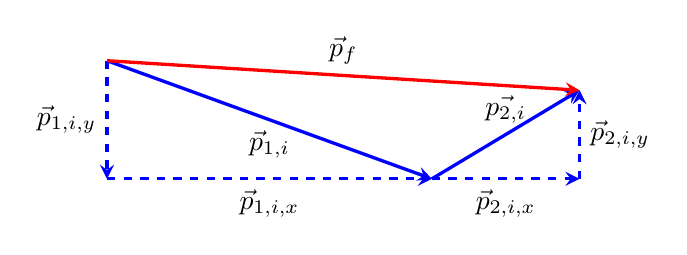
\begin{tikzpicture}[scale=1.5]
        \draw (0,0) coordinate (o) node[above]{};
        \draw (0,1) coordinate (a) node[above]{};
        \draw (2.75,0) coordinate (b) node[above]{};
        \draw (4,0) coordinate (c) node[above]{};
        \draw (4,0.75) coordinate (d) node[above]{};

        \draw[->,very thick,draw=blue,dashed,-stealth] (a)--node[left]{$\vec{p}_{1,i,y}$}(o);
        \draw[->,very thick,draw=blue,dashed,-stealth] (o)--node[below]{$\vec{p}_{1,i,x}$}(b);
        \draw[->,very thick,draw=blue,-stealth] (a)--node[below]{$\vec{p}_{1,i}$}(b);
        \draw[->,very thick,draw=blue,dashed,-stealth] (c)--node[right]{$\vec{p}_{2,i,y}$}(d);
        \draw[->,very thick,draw=blue,dashed,-stealth] (b)--node[below]{$\vec{p}_{2,i,x}$}(c);
        \draw[->,very thick,draw=blue,-stealth] (b)--node[above]{$\vec{p_{2,i}}$}(d);
        \draw[->,very thick,draw=red,-stealth] (a)--node[above]{$\vec{p}_f$}(d);
    \end{tikzpicture}
    \item Add $x$ and $y$ components to obtain $x$ and $y$ components of final momentum\\
    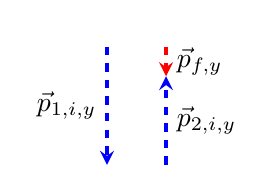
\begin{tikzpicture}[scale=1.5]
        \draw (-0.25,0) coordinate (a) node[above]{};
        \draw (0.25,0) coordinate (b) node[above]{};
        \draw (-0.25,1) coordinate (c) node[above]{};
        \draw (0.25,0.75) coordinate (d) node[above]{};
        \draw (0.25, 1) coordinate (e) node[above]{};

        \draw[->,very thick,draw=blue,dashed,-stealth] (c)--node[left]{$\vec{p}_{1,i,y}$}(a);
        \draw[->,very thick,draw=blue,dashed,-stealth] (b)--node[right]{$\vec{p}_{2,i,y}$}(d);
        \draw[->,very thick,draw=red,dashed,-stealth] (e)--node[right]{$\vec{p}_{f,y}$}(d);
    \end{tikzpicture}\\
    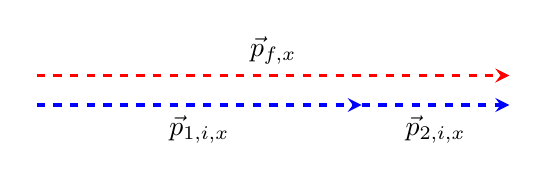
\begin{tikzpicture}[scale=1.5]
        \draw (-2,0) coordinate (a) node[above]{};
        \draw (2,0) coordinate (b) node[above]{};
        \draw (-2,-0.25) coordinate (c) node[above]{};
        \draw (0.75,-0.25) coordinate (d) node[above]{};
        \draw (2,-0.25) coordinate (e) node[above]{};

        \draw[->,very thick,draw=red,dashed,-stealth] (a)--node[above]{$\vec{p}_{f,x}$}(b);
        \draw[->,very thick,draw=blue,dashed,-stealth] (c)--node[below]{$\vec{p}_{1,i,x}$}(d);
        \draw[->,very thick,draw=blue,dashed,-stealth] (d)--node[below]{$\vec{p}_{2,i,x}$}(e);
    \end{tikzpicture}
    \item Add $x$ and $y$ components to obtain $x$ and $y$ components of final momentum\\
    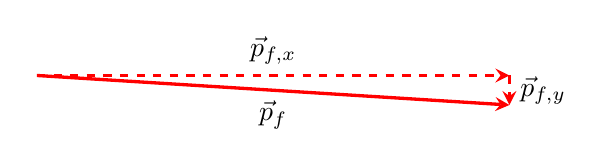
\begin{tikzpicture}[scale=1.5]
        \draw (0,0) coordinate (a) node[above]{};
        \draw (4,0) coordinate (b) node[above]{};
        \draw (4,-0.25) coordinate (c) node[above]{};

        \draw[->,very thick,draw=red,dashed,-stealth] (a)--node[above]{$\vec{p}_{f,x}$}(b);
        \draw[->,very thick,draw=red,dashed,-stealth] (b)--node[right]{$\vec{p}_{f,y}$}(c);
        \draw[->,very thick,draw=red,-stealth] (a)--node[below]{$\vec{p}_f$}(c); 
    \end{tikzpicture}
\end{enumerate}
Each of these component equations are solved independently to obtain $x$ and $y$ components of the desired velocity vector (here $m$ represents the total mass of the system)
\begin{align*}
    v_{f,x} &= \frac{m_1 v_{1,i,x} + m_2 v_{2,i,x}}{m}\\
    v_{f,y} &= \frac{m_1 v_{1,i,y} + m_2 v_{2,i,y}}{m}
\end{align*}
Finally, combine these components using Pythagorean theorem
\begin{align*}
    v_f = |\vec{v}_f| = \sqrt{v^2_{f,x} + v^2_{f,y}}
\end{align*}

\begin{shaded}
    \underline{\bf{Problem-Solving Strategy:} Conservation of Motion in 2D}
    \vspace{2mm}\\
    The method for solving a 2D (or 3D) conservation of momentum problem is generally the same as for 1D.
    \begin{enumerate}
        \item Identify a closed system
        \item Write down the equation that represents conservation of momentum in the $x$ direction and solve for the desired quantity. This will give you the $x$ component of the vector
        \item Write down the equation that represents conservation of momentum in the $y$ direction and solve. This will give you the $y$ component of the vector
        \item Assuming you are calculating a vector quantity, use Pythagorean theorem to calculate its magnitude
    \end{enumerate}
\end{shaded}

\begin{shaded}
    \underline{\bf{Example 9.14:} Traffic Collision}
    \vspace{2mm}\\
    A small car of mass $m_c = 1200$ kg travelling east at $v_c = 60$ kmh$^{-1}$ collides at an intersection with a truck of mass $m_T = 3000$ kg that is traveling north at $v_T = 40$ kmh$^{-1}$. The two vehicles are locked together, what is the velocity of the combined wreckage?
    \vspace{1mm}\\
    Before the collision the total momentum is:\ $\displaystyle \vec{p} = m_c\vec{v}_c + m_T\vec{v}_T$\\
    After the collision the wreckage has momentum:\ $\displaystyle \vec{p} = (m_c + m_T)\vec{v}_w$\\
    Since the system is closed, momentum is conserved:\ $\displaystyle m_c\vec{v}_c + m_T\vec{v}_T = (m_c + m_T)\vec{v}_w$\\
    The two initial momenta are not parallel and must be added as vectors
    \begin{center}
        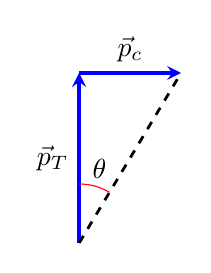
\begin{tikzpicture}[scale=0.5]
            \draw (0,0) coordinate (a);
            \draw (0,4.32) coordinate (b);
            \draw (2.59,4.32) coordinate (c);
            \draw (2.59,0) coordinate (d);

            \draw[->,very thick,draw=blue,-stealth] (a)--node[left]{$\vec{p}_T$}(b);
            \draw[->,very thick,draw=blue,-stealth] (b)--node[above]{$\vec{p}_c$}(c);
            \draw[line width=1pt,dashed] (a)--(c);
            \draw pic["$\theta$", draw=red, -, angle eccentricity=1.3, angle radius=0.75cm]{angle=c--a--b};
        \end{tikzpicture}
    \end{center}
    If the $+x$ direction is defined to point east, and the $+y$ direction is defined to point north, then:
    \begin{align*}
        \vec{p}_c &= p_c\hat{i} = m_c v_c \hat{i}\\
        \vec{p}_T &= p_T\hat{j} = m_T v_T \hat{j}
    \end{align*}
    Therefor in the $x$ direction and $y$ direction respectively:\\
    \begin{minipage}{0.45\textwidth}
        \begin{align*}
            m_cv_c &= (m_c + m_T)v_{w,x}\\
            v_{w,x} &= \bigg(\frac{m_c}{m_c + m_T}\bigg)v_c
        \end{align*}
    \end{minipage}
    \begin{minipage}{0.45\textwidth}
        \begin{align*}
            m_Tv_T &= (m_c + m_T)v_{w,y}\\
            v_{w,y} &= \bigg(\frac{m_T}{m_c + m_T}\bigg)v_T
        \end{align*}
    \end{minipage}
    \vspace{2mm}\\
    Applying Pythagorean theorem gives:
    \begin{align*}
        |\vec{v}_w| &= \sqrt{\bigg[\bigg(\frac{m_c}{m_c + m_T}\bigg)v_c\bigg]^2 + \bigg[\bigg(\frac{m_T}{m_c + m_T}\bigg)v_T\bigg]^2}\\
        &= \sqrt{\bigg[\bigg(\frac{1200\text{ kg}}{4200\text{ kg}}\bigg)\Big(16.67\text{ ms}^{-1}\Big)\bigg]^2 + \bigg[\bigg(\frac{3000\text{ kg}}{4200\text{ kg}}\bigg)\Big(11.1\text{ ms}^{-1}\Big)\bigg]^2}\\
        &= \sqrt{\Big(4.76\text{ ms}^{-1}\Big)^2 + \Big(7.93\text{ ms}^{-1}\Big)^2}\\
        &= 9.25\text{ ms}^{-1}\\
        &\approx 33.3\text{ kmh}^{-1}
    \end{align*}
    As for its direction, using the angle $\theta$:
    \begin{align*}
        \theta = \tan^{-1}\bigg(\frac{v_{w,x}}{v_{w,y}}\bigg)\ \boldsymbol{\to}\ \tan^{-1}\bigg(\frac{4.76\text{ ms}^{-1}}{7.93\text{ ms}^{-1}}\bigg) = 31\degree
    \end{align*}
    This angle is $31\degree$ east of north, or $59\degree$ counterclockwise with respect to $+x$
\end{shaded}

\subsection{Center of Mass}
\bf{Internal \& External Forces}
\vspace{2mm}\\
Suppose we have an extended object of mass $M$, made of $N$ interacting particles of masses $m_j$:
\begin{equation}
    M = \sum_{j = 1}^{N}m_j
\end{equation}
If we apply a net external force $\vec{F}_{ext}$ on the object, every possible particle experiences spme fraction of that external force. Let
\begin{center}
    $\vec{f}^{ext}_j =$ the fraction of the external force that the $j^{\text{th}}$ particle experiences
\end{center}
These fractions of the total force are not necessarily equal, they virtually never are. In general:
\begin{align*}
    \vec{f}^{ext}_1 \neq \vec{f}^{ext}_2 \neq ... \neq \vec{f}^{ext}_N
\end{align*}
Assume that each particle making up the object can interact with every other particle of the object, these are internal forces, $\vec{f}^{int}_j$ = the net internal force that the $j^{\text{th}}$ particle experiences from all the other particles in the object. The net force on the $j^{\text{th}}$ particle is the vector sum of these:
\begin{align}
    \vec{f}_j = \vec{f}^{int}_j + \vec{f}^{ext}_j
\end{align}
As a result of this fractional force, the momentum of each particle gets changed:
\begin{align}
    \begin{split}
        \vec{f}_j &= \frac{d\vec{p}_j}{dt}\\
        \vec{f}^{int}_j + \vec{f}^{ext}_j &= \frac{d\vec{p}_j}{dt}
    \end{split}
\end{align}
The net force $\vec{F}$ on the object is the vector sum of these forces:
\begin{align}
    \begin{split}
        \vec{F}_{net} &= \sum_{j = 1}^{N}\bigg(\vec{f}^{int}_j + \vec{f}^{ext}_j\bigg)\\
        &= \sum_{j = 1}^{N}\vec{f}^{int}_j + \sum_{j = 1}^{N}\vec{f}^{ext}_j
    \end{split}
\end{align}
The net force changes the momentum of the object as a whole, and the net change of momentum of the object must be the vector sum of all the individual changes of momentum of all the particles:
\begin{equation}
    \vec{F}_{net} = \sum_{j = 1}^{N}\frac{d\vec{p}_j}{dt}
\end{equation}
Combining the two previous equations gives:
\begin{equation}
    \sum_{j = 1}^{N}\vec{f}^{int}_j + \sum_{j = 1}^{N}\vec{f}^{ext}_j = \sum_{j = 1}^{N}\frac{d\vec{p}_j}{dt}
\end{equation}
In general, the internal forces for any individual part of the object won't cancel, but when all of the internal forces are summed, the internal forces must cancel in pairs. The sum of all the internal forces must be zero.
\begin{align*}
    \sum_{j = 1}^{N}\vec{f}^{int}_j = 0
\end{align*}
For the external forces, this summation is simply the total external force applied to the whole object:
\begin{align*}
    \sum_{j = 1}^{N}\vec{f}^{ext}_j = \vec{F}_{ext}
\end{align*}
As a result:
\begin{equation}
    \vec{F}_{ext} = \sum_{j = 1}^{N}\frac{d\vec{p}_j}{dt}
\end{equation}
This equation shows that the total change of momentum of the entire object (all $N$ particles) is due only to external forces, internal forces do not change the momentum of the object as a whole. (This the reason "pull yourself up by your bootstraps" is impossible, upward pulling is an internal force)
\vspace{2mm}\\
\bf{Force \& Momentum}
\vspace{2mm}\\
The goal is to determine the equation of motion for the entire object (the entire system of particles). $\vec{p}_{cm}$ is the total momentum of the system of $N$ particles, and is defined:
\begin{align*}
    \vec{p}_{cm} = \sum_{j = 1}^{N}\vec{p}_j
\end{align*}
Therefore, equation 25 can be written simply as:
\begin{equation}
    \vec{F} = \frac{d\vec{p}_{cm}}{dt}
\end{equation}
Because the change in momentum is caused only by the net external force, the "ext" subscript has been dropped. Equation 26 is Newton's second law for the entire extended object

\newpage
\noindent\bf{Center of Mass}
\vspace{2mm}\\
If $M$ is the mass of the combined system of particles, then:
\begin{equation}
    \vec{F} = M\vec{a}
\end{equation}
Equating with equation 26 gives:
\begin{align*}
    M\vec{a} &= \frac{d\vec{p}_{cm}}{dt}\\
    M\vec{a} &= \sum_{j = 1}^{N}\frac{d\vec{p}_j}{dt} = \frac{d}{dt}\sum_{j = 1}^{N}\vec{p}_j
\end{align*}
Which follows because the derivative of a sum is equal to the sum of the derivatives.
\vspace{1mm}\\
Now, $\vec{p}_j$ is the momentum of the $j^{th}$ particle. Defining the positions of the constituent particles as $\vec{r} = (x_j, y_j, z_j)$ we have:
\begin{align*}
    \vec{p}_j = m_j\vec{v}_j = m_j\frac{d\vec{r}_j}{dt}
\end{align*}
Substituting that back into the previous equation gives:
\begin{align*}
    M\vec{a} &= \frac{d}{dt}\bigg(\sum_{j = 1}^{N}m_j\frac{d\vec{r}_j}{dt}\bigg)\\
    &= \frac{d^2}{dt^2}\bigg(\sum_{j = 1}^{N}m_j\vec{r}_j\bigg)
\end{align*}
Dividing both sides by $M$ - the total mass of the system of particles - gives:
\begin{equation}
    \vec{a} = \frac{d^2}{dt^2}\bigg(\frac{1}{M}\sum_{j = 1}^{N}m_j\vec{r}_j\bigg)
\end{equation}
Inside the parentheses this equation calculates the product of each particle's mass with its position, sums all $N$ of these up, and divides by the total mass of the particles that were summed. This can be interpreted as the weighted average position of the mass of an extended object or its \bf{center of mass}. The position of the center of mass has units of meters, suggesting a definition:
\begin{equation}
    \vec{r}_{cm} = \frac{1}{M}\sum_{j = 1}^{N}m_j\vec{r}_j
\end{equation}
The point that obeys equation 26 and 27 is the center of mass of the object, located at the position vector $\vec{r}_cm$. There does not have to be any actual mass at the center of mass of an object. A hollow steel sphere with a vacuum inside is spherically symmetrical, its mass is uniformly distributed about the center. All of the mass is on the surface, with none inside however, it can be shown that its center of mass is at its geometric center.


\begin{minipage}{0.45\textwidth}
    \begin{enumerate}
        \item[(a)] Position vectors are created for each object \newline
        ($\vec{r}_1$, $\vec{r}_2$, $\vec{r}_3$) object\\
        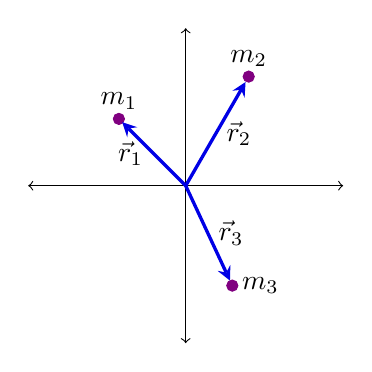
\begin{tikzpicture}[scale=2]
            %%% COORDINATES %%%
            \draw (0,0) coordinate (O);
            \draw ({-0.6*cos(45)},{0.6*sin(45)}) coordinate (m1);
            \draw ({0.8*cos(60)},{0.8*sin(60)}) coordinate (m2);
            \draw ({0.7*cos(65)},{-0.7*sin(65)}) coordinate (m3);
    
            %%% POINTS %%%
            \filldraw[violet] (m1) circle (1pt) node[above,text=black]{$m_1$};
            \filldraw[violet] (m2) circle (1pt) node[above,text=black]{$m_2$};
            \filldraw[violet] (m3) circle (1pt) node[right,text=black]{$m_3$};
    
            %%% AXES %%%
            \draw[<->] (-1,0)--(1,0);
            \draw[<->] (0,-1)--(0,1);
    
            %%% VECTORS %%%
            \draw[->,very thick,-stealth,draw=black!10!blue] (O)--node[left]{$\vec{r}_1$}({-0.57*cos(45)},{0.57*sin(45)});
            \draw[->,very thick,-stealth,draw=black!10!blue] (O)--node[right]{$\vec{r}_2$}({0.76*cos(60)},{0.76*sin(60)});
            \draw[->,very thick,-stealth,draw=black!10!blue] (O)--node[right]{$\vec{r}_3$}({0.665*cos(65)},{-0.665*sin(65)});
        \end{tikzpicture}
        \item[(c)] The scaled vectors are added together\\
        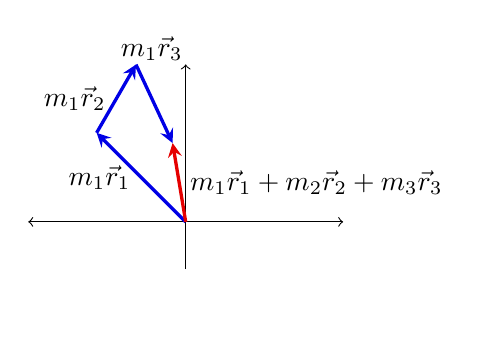
\begin{tikzpicture}[scale=2]
            %%% COORDINATES %%%
            \draw (0,0) coordinate (O);
            \draw ({-0.6*cos(45)},{0.6*sin(45)}) coordinate (m1);
            \draw ({0.8*cos(60)},{0.8*sin(60)}) coordinate (m2);
            \draw ({0.7*cos(65)},{-0.7*sin(65)}) coordinate (m3);
            
            %%% AXES %%%
            \draw[<->] (-1,0)--(1,0);
            \draw[->] (0,-0.3)--(0,1);
    
            %%% VECTORS %%%
            \draw[->,very thick,-stealth,draw=black!10!blue] (O)--node[left]{$m_1\vec{r}_1$}({-0.8*cos(45)},{0.8*sin(45)});
            \draw[->,very thick,-stealth,draw=black!10!blue] ({-0.8*cos(45)},{0.8*sin(45)})--node[left]{$m_1\vec{r}_2$}([turn]-75:0.5);
            \draw[->,very thick,-stealth,draw=black!10!blue]  ({(-0.8*cos(45)) + 0.5*cos(60)},{(0.8*sin(45)) + (0.5*sin(60))})--({-0.8*cos(45) + (0.5*cos(60)) + (0.55*cos(65))} , {(0.8*sin(45)) + (0.5*sin(60)) - (0.55*sin(65))});
            \node at ({(-0.8*cos(45)) + 0.5*cos(60) + 0.1},{(0.8*sin(45)) + (0.5*sin(60)) + 0.1}){$m_1\vec{r}_3$};
            \draw[->,very thick,-stealth,draw=black!10!red] (O)--node[right]{$m_1\vec{r}_1 + m_2\vec{r}_2 + m_3\vec{r}_3$} ({-0.8*cos(45) + (0.5*cos(60)) + (0.55*cos(65))} , {(0.8*sin(45)) + (0.5*sin(60)) - (0.55*sin(65))});
        \end{tikzpicture}
    \end{enumerate}
\end{minipage}
\begin{minipage}{0.45\textwidth}
    \begin{enumerate}
        \item[(b)]\vspace{1.8mm}
        The position vectors are multiplied by the mass of the corresponding object\\
        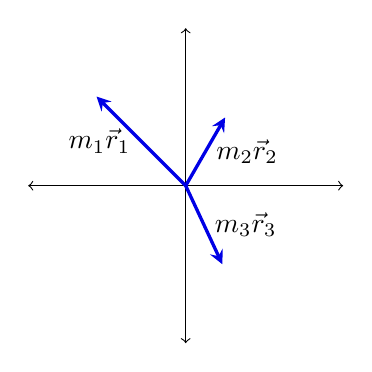
\begin{tikzpicture}[scale=2]
            %%% COORDINATES %%%
            \draw (0,0) coordinate (O);
            \draw ({-0.6*cos(45)},{0.6*sin(45)}) coordinate (m1);
            \draw ({0.8*cos(60)},{0.8*sin(60)}) coordinate (m2);
            \draw ({0.7*cos(65)},{-0.7*sin(65)}) coordinate (m3);
            
            %%% AXES %%%
            \draw[<->] (-1,0)--(1,0);
            \draw[<->] (0,-1)--(0,1);
            %% 0.8 + 0.5 + 0.55
            %%% VECTORS %%%
            \draw[->,very thick,-stealth,draw=black!10!blue] (O)--node[left]{$m_1\vec{r}_1$}({-0.8*cos(45)},{0.8*sin(45)});
            \draw[->,very thick,-stealth,draw=black!10!blue] (O)--node[right]{$m_2\vec{r}_2$}({0.5*cos(60)},{0.5*sin(60)});
            \draw[->,very thick,-stealth,draw=black!10!blue] (O)--node[right]{$m_3\vec{r}_3$}({0.55*cos(65)},{-0.55*sin(65)});
        \end{tikzpicture}
        \item[(d)] The final vector is divided by the total mass.\\
        \begin{tikzpicture}[scale=2]
            %%% AXES %%%
            \draw[<->] (-1,0)--(1,0);
            \draw[->] (0,-0.3)--(0,1);
    
            %%% VECTORS %%%
            \draw[->,very thick,-stealth,draw=black!10!red] (O)--({0.67419*((-0.8*cos(45)) + (0.5*cos(60)) + (0.55*cos(65)))} , {0.67419*((0.8*sin(45)) + (0.5*sin(60)) - (0.55*sin(65)))});
            \node at (0.85,0.25){$\displaystyle \frac{m_1\vec{r}_1 + m_2\vec{r}_2 + m_3\vec{r}_3}{m_1 + m_2 + m_3}$};
        \end{tikzpicture}\\
        This vector is $\vec{r}_{cm}$ and points to the center of mass of the system (no mass is actually present at the center of mass of the system)
    \end{enumerate}
\end{minipage}
\newpage
\noindent Since $\vec{r}_j = x_j\hat{i} + y_j\hat{j} + z_j\hat{k}$, it follows that:
\begin{align}
    r_{cm,x} &= \frac{1}{M}\sum_{j = 1}^{N}m_jx_j\\
    r_{cm,y} &= \frac{1}{M}\sum_{j = 1}^{N}m_jy_j\\
    r_{cm,z} &= \frac{1}{M}\sum_{j = 1}^{N}m_jz_j
\end{align}
Thus, 
\begin{align*}
    \vec{r}_{cm} = r_{cm,x}\hat{i} + r_{cm,y}\hat{j} + r_{cm,z}\hat{k}\\
    r_{cm} = |\vec{r}_{cm}| = \Big(r^2_{cm,x} + r^2_{cm,y} + r^2_{cm,z}\Big)^{\sfrac{1}{2}}
\end{align*}
Therefore, the components of the center of mass vector can be calculated individually. The instantaneous velocity of the center of mass is calculated by taking the derivative of $\vec{r}_{cm}$
\begin{equation}
    \vec{v}_{cm} = \frac{d}{dt}\bigg(\frac{1}{M}\sum_{j = 1}^{N}m_j\vec{r}_j\bigg) = \frac{1}{M}\sum_{j = 1}^{N}m_j\vec{v}_j
\end{equation}

\begin{shaded}
    \underline{\bf{Example 9.16:} Center of Mass of the Earth-Moon System}
    \vspace{2mm}\\
    Using data from the text appendix, determine how far the center of mass of the Earth-Moon system is from the center of Earth. Compare this distance to the radius of Earth.
    \vspace{1mm}\\
    From Appendix D: $m_e = 5.97 \cdot 10^{24}$ kg, $m_m = 7.36 \cdot 10^{22}$ kg, $r_m = 3.82 \cdot 10^{8}$ m
    \vspace{1mm}\\
    Define the origin of the coordinate system as the center of Earth, with two objects, equation 29 becomes:
    \begin{align*}
        R = \frac{m_e r_e + m_m r_m}{m_e + m_m}
    \end{align*}
    The center of the Earth was defined as the origin so $r_e = 0$ m. Substituting the above values into the equation for $R$ gives:
    \begin{align*}
        R &= \frac{(5.97 \cdot 10^{24}\text{ kg})(0\text{ m}) + (7.36 \cdot 10^{22}\text{ kg})(3.82 \cdot 10^8\text{ m})}{(5.97 \cdot 10^{24}\text{ kg}) + (7.36 \cdot 10^{22}\text{ kg})}\\
        R &= 4.64 \cdot 10^6\text{ m}
    \end{align*}
    The radius of the Earth is $6.37 \cdot 10^6$ m, so the center of mass of the Earth-Moon system is $(6.37 - 4.64) \cdot 10^6$ m $= 1.73 \cdot 10^6$ m = 1730 km below the surface of the Earth
\end{shaded}

\noindent\bf{Center of Mass of Continuous Objects}
\vspace{2mm}\\
If the object in question, has its mass distributed uniformly in space, rather than as a collection of discreet particles, then $m_j \to dm$, and the summation becomes an integral:
\begin{equation}
    \vec{r}_{cm} = \frac{1}{M}\int\vec{r}dm
\end{equation}
In this context $r$ is a characteristic dimension of the object. To generate an integrand that can actually be calculated, the differential mass element $dm$ must be expressed as a function of the mass density of the continuous object, and the dimension $r$. This is clarified in the following example.

\newpage
\begin{shaded}
    \underline{\bf{Example 9.18:} Center of Mass of a Uniform Thin Hoop}
    \vspace{2mm}\\
    Because of the hoop's symmetry, its center of mass should be at its geometric center. Defining the coordinate system such that the origin is located at the center of the hoop, the integral should evaluate to zero.
    \vspace{1mm}\\
    We replace $dm$ with an expression involving the density of the hoop and the radius of the hoop to create an expression that can be integrated. We treat the hoop as a 1D object, its density is expressed as the number of $\sfrac{\text{kg}}{\text{m}}$. This kind of density is called \bf{linear mass density} and is given the symbol $\lambda$.
    \vspace{1mm}\\
    Because the hoop is described as uniform, the linear mass density $\lambda$ is constant. To get an expression for the differential mass element $dm$, we multiply $\lambda$ by a differential length of the hoop, substitute, and integrate (with appropriate limits for the definite integral).\\
    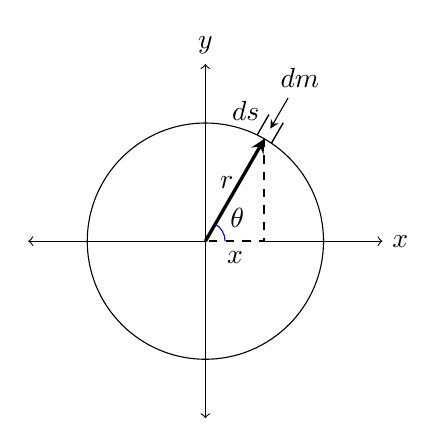
\begin{tikzpicture}[scale=1.5]
        %%% AXES %%%
        \draw[<-] (-1.5,0)--(0,0);
        \draw[->] ({cos(60)},0)--(1.5,0) node[right]{$x$};
        \draw[<->] (0,-1.5)--(0,1.5) node[above]{$y$};
        \draw (0,0) circle (1);

        %%% COORDINATES %%%
        \draw (0,0) coordinate (O);
        \draw ({cos(60)},{sin(60)}) coordinate (a) node{};
        \draw ({cos(60)},0) coordinate (b) node{};

        %%% ARC dm %%%
        \centerarc[red,very thick](0,0)(56:64:1);

        %%% LINES %%%
        \draw[->,very thick,-stealth] (O)--node[left,xshift=1.2mm,yshift=1mm]{$r$}(a);
        \draw[line width=0.75pt,dashed] (a)--(b)--node[below]{$x$}(O);
        \draw pic[draw=blue, -, angle eccentricity=2, angle radius=0.25cm]{angle=b--O--a};
        \node at (0.27,0.2){$\theta$};

        %%% ds LINE %%%
        \draw[line width=0.5pt] ({cos(64)},{sin(64)})--node[left,xshift=0.8mm,yshift=1.8mm]{$ds$}({(cos(64) + 0.2*cos(60))},{(sin(64) + 0.2*sin(60))});
        \draw[line width=0.5pt] ({cos(56)},{sin(56)})--({(cos(56) + 0.2*cos(60))},{(sin(56) + 0.2*sin(60))});

        \draw[->,-stealth] ({1.4*cos(60)},{1.4*sin(60)})--({1.1*cos(60)},{1.1*sin(60)});
        \node at ({1.6*cos(60)},{1.6*sin(60)}){$dm$};
    \end{tikzpicture}\\
    The center of mass is calculated with equation 34:
    \begin{align*}
        \displaystyle \vec{r}_{cm} = \frac{1}{M} \int_{a}^{b}\vec{r}dm 
    \end{align*}
    We need to determine the limits of integration $a$ and $b$. The piece of the hoop of differential length $ds$ has a differential mass $dm = \lambda ds$, substituting in and expressing $\vec{r}$ in component form gives:
    \begin{align*}
        \vec{r}_{cm} &= \frac{1}{M}\int_{a}^{b} \Big[(r\cos(\theta))\hat{i} + (r\sin(\theta))\hat{j}\Big]dm\\
        \vec{r}_{cm} &= \frac{1}{M}\int_{a}^{b} \Big[(r\cos(\theta))\hat{i} + (r\sin(\theta))\hat{j}\Big]\lambda ds
    \end{align*}
    The arc length $ds$ subtends a different angle $d\theta$ so we have $ds = rd\theta$, thus:
    \begin{align*}
        \vec{r}_{cm} = \frac{1}{M}\int_{a}^{b} \Big[(r\cos(\theta))\hat{i} + (r\sin(\theta))\hat{j}\Big]\lambda rd\theta
    \end{align*}
    Since $\lambda$ is the linear mass density, it is computed by dividing the total mass by the length of the hoop: $\displaystyle \lambda = \frac{M}{2\pi r}$\\
    This gives us:
    \begin{align*}
        \vec{r}_{cm} &= \frac{1}{M}\int_{a}^{b} \Big[(r\cos(\theta))\hat{i} + (r\sin(\theta))\hat{j}\Big]\bigg(\frac{M}{2\pi r}\bigg) rd\theta\\
        &= \frac{1}{2\pi}\int_{a}^{b} \Big[(r\cos(\theta))\hat{i} + (r\sin(\theta))\hat{j}\Big] d\theta
    \end{align*}
    The variable of integration is now the angle $\theta$. This tells us that the limits of integration are $\theta = 0$ to $\theta = 2\pi$, so $a = 0$ \& $b = 2\pi$
    \begin{align*}
        \vec{r}_{cm} &= \frac{1}{2\pi}\int_{0}^{2\pi} \Big[(r\cos(\theta))\hat{i} + (r\sin(\theta))\hat{j}\Big] d\theta\\
        \vec{r}_{cm} &= r_{cm,x}\hat{i} + r_{cm,y}\hat{j}\\
        &= \bigg[\frac{1}{2\pi}\int_{0}^{2\pi}\big(r\cos(\theta)\big)d\theta\bigg]\hat{i} + \bigg[\frac{1}{2\pi}\int_{0}^{2\pi}\big(r\sin(\theta)\big)d\theta\bigg]\hat{j}\\
        &= 0\hat{i} + 0\hat{j} = \vec{0}
    \end{align*}
\end{shaded}
\newpage

\noindent\bf{Center of Mass and Conservation of Momentum}
\vspace{2mm}\\
Suppose you have $N$ objects with masses $m_1, m_2, m_3, ... m_N$ and initial velocities $\vec{v}_1, \vec{v}_2, \vec{v}_3, ... \vec{v}_N$, the center of mass of the object is given by
\begin{align*}
    \vec{r}_{cm} = \frac{1}{M}\sum_{j = 1}^{N}m_j\vec{r}_j
\end{align*}
Its velocity is:
\begin{equation}
    \vec{v}_{cm} = \frac{d\vec{r}_{cm}}{dt} = \frac{1}{M}\sum_{j = 1}^{N}m_j\frac{d\vec{r}_j}{dt}
\end{equation}
And thus, the initial momentum of the center of mass is:
\begin{align*}
    \bigg[M\frac{d\vec{r}_{cm}}{dt}\bigg]_i &= \sum_{j = 1}^{N}m_j\frac{d\vec{r}_{j,i}}{dt}\\
    M\vec{v}_{cm,i} &= \sum_{j = 1}^{N}m_j\vec{v}_{j,i}
\end{align*}
After these masses move and interact with each other, the momentum of the center of mass is
\begin{align*}
    M\vec{v}_{cm,f} &= \sum_{j = 1}^{N}m_j\vec{v}_{j,f}
\end{align*}
Conservation of momentum tells us that the right hand side of both equations must be equal, which says:
\begin{equation}
    M\vec{v}_{cm,f} = M\vec{v}_{cm,i}
\end{equation}
This implies that conservation of momentum is expressed in terms of the center of mass of the system. An individual particle of the object may accelerate in various directions with various magnitudes depending on the net internal force acting on the object. Such a particle's momentum will not be constant, but the momentum of the entire extended object will be.\par
Since $M$ represents the mass of the entire system of particles, it is necessarily constant. As a result, equation 36 implies that for a closed system:
\begin{equation}
    \vec{v}_{cm,f} = \vec{v}_{cm,i}
\end{equation}
In other words, in the absence of an external force, the velocity of the center of mass never changes

\end{document}